\documentclass[12pt,a4paper]{article}
%\DeclareMathSizes{12}{14}{10}{6}
\usepackage[utf8]{inputenc}
\usepackage[T1]{fontenc}
\usepackage[english]{babel}
\usepackage[outer=25mm,inner=35mm,top=25mm,bottom=25mm]{geometry}

\usepackage{indentfirst}
\usepackage{colortbl}
\usepackage{amsmath}
\usepackage{caption}
\usepackage{graphicx}
\usepackage{setspace}
\usepackage{hyperref}
\usepackage[export]{adjustbox}
\usepackage{listings}
\usepackage{wrapfig}
\usepackage{float}
\usepackage[
backend=biber,
style=mla,
sorting=ynt
]{biblatex}
\usepackage{optidef}
\addbibresource{ref.bib}

\frenchspacing
\linespread{1.5}

\begin{document}
	\noindent {\Large Corvinus University of Budapest\\
		Institute of Economics}\\
	
	\vspace{35mm}
	
	\begin{center}
		{\huge The asymmetric effect of uncertainty on monetary transmission}\\
	\end{center}
	
	\vspace{90mm}
	
	\begin{flushright}
		{\Large Péter Horváth}\\
		%{\Large Makrogazdasági- és piacelemző szakirány}\\
		{\Large 2022}
	\end{flushright}
	
	\vspace{10mm}
	\begin{center}
		{\Large Supervisor : István Kónya}
	\end{center}
	
	\thispagestyle{empty}
	
	\pagebreak
	\setcounter{tocdepth}{2}
%	\tableofcontents
	%\listoftables
	%\listoffigures
	
	\pagebreak
\begin{center} \section*{Abstract} \end{center}

This paper discusses the asymmetric effect of uncertainty on the monetary transmission mechanism. The notion is that during periods characterized by high uncertainty spikes, the transmission mechanism of the interest rate channel is less effective, thus implying the importance of using forward guidance alongside interest rate decisions. To study this nonlinear relationship, I use a rolling window approach to estimate sign restricted VAR models over these periods in question. The results of the estimation show a minor difference in the impact of an interest rate shock during high-uncertainty periods, compared to the estimate over the whole time series.\\

\bigskip

\noindent \textbf{Keywords:} Uncertainty, Monetary transmission, Asymmetry, Sign restriction, Vector-Autoregression

\pagebreak

\section{Introduction}
Over the recent years, uncertainty and asymmetries are two subjects that gained considerable traction in macroeconomics research. Both fields of research already have a rich literature, with there being a consensus on uncertainty shocks having an impact resembling that of a negative demand shock on economic activity (\textcolor{blue}{\cite{CARRIERESWALLOW2013316}}, \textcolor{blue}{\cite{COLOMBO201339}}, \textcolor{blue}{\cite{CALDARA2016185}}, \textcolor{blue}{\cite{CHENG2018305}}, \textcolor{blue}{\cite{BONCIANI2020102236}}, \textcolor{blue}{\cite{NILAVONGSE2020108765}}); and several papers have shown that macroeconomic shocks can have different impacts depending on the state of the economy.
\textcolor{blue}{\cite{RePEc:eee:jmacro:v:69:y:2021:i:c:s0164070421000379}}, \textcolor{blue}{\cite{RePEc:fip:fedker:00016}}, \textcolor{blue}{\cite{RePEc:cup:macdyn:v:20:y:2016:i:05:p:1219-124600}} and \textcolor{blue}{\cite{RePEc:jae:japmet:v:19:y:2004:i:5:p:551-565}} all take slightly different approaches, however all papers find that the impact of (negative) macroeconomic shocks is a sharper decline when uncertainty is high. Similar processes can be observed when carrying out the analysis with respect to the economy's position in the business cycle. \textcolor{blue}{\cite{RePEc:knz:dpteco:1402}} and \textcolor{blue}{\cite{RePEc:een:camaaa:2020-72}} show that uncertainty shocks have larger impact during economic contractions, and \textcolor{blue}{\cite{RePEc:gro:rugsom:98c36}} finds that monetary transmission is amplified during recessionary periods in the US and Germany. Another field of research on asymmetric dynamics is finding asymmetry in monetary policy-making itself. \textcolor{blue}{\cite{Lin+2021+425+447}} finds that macroeconomic aggregates react asymmetrically to positive and negative monetary policy shocks. \textcolor{blue}{\cite{doi:10.1080/1331677X.2018.1481445}} links uncertainty and asymmetries in monetary policy by assuming a difference in the policy reaction function in over the business cycle. \\

With this paper, I aim to contribute to the pre-existing literature, by linking the effect of uncertainty to the efficacy of monetary transmission. The results could have key implications for policy making, more specifically, it could highlight the importance of forward guidance measures, especially during times, when economic uncertainty is at its peak. \\

The rest of the paper will be outlined as follows: Section 2 gives a brief overview of the data used, Section 3 discusses the empirical strategy, in Section 4 I discuss the results and Section 5 concludes.

\section{Data}

For the purposes of the analysis I will be estimating VAR models with three variables, the federal funds rate, consumer price index, and industrial production index. All data are monthly from ranging from January 1985 to December 2019 and all are retrieved from the federal reserve database. \\

\begin{center}
\begin{figure}[h!]
	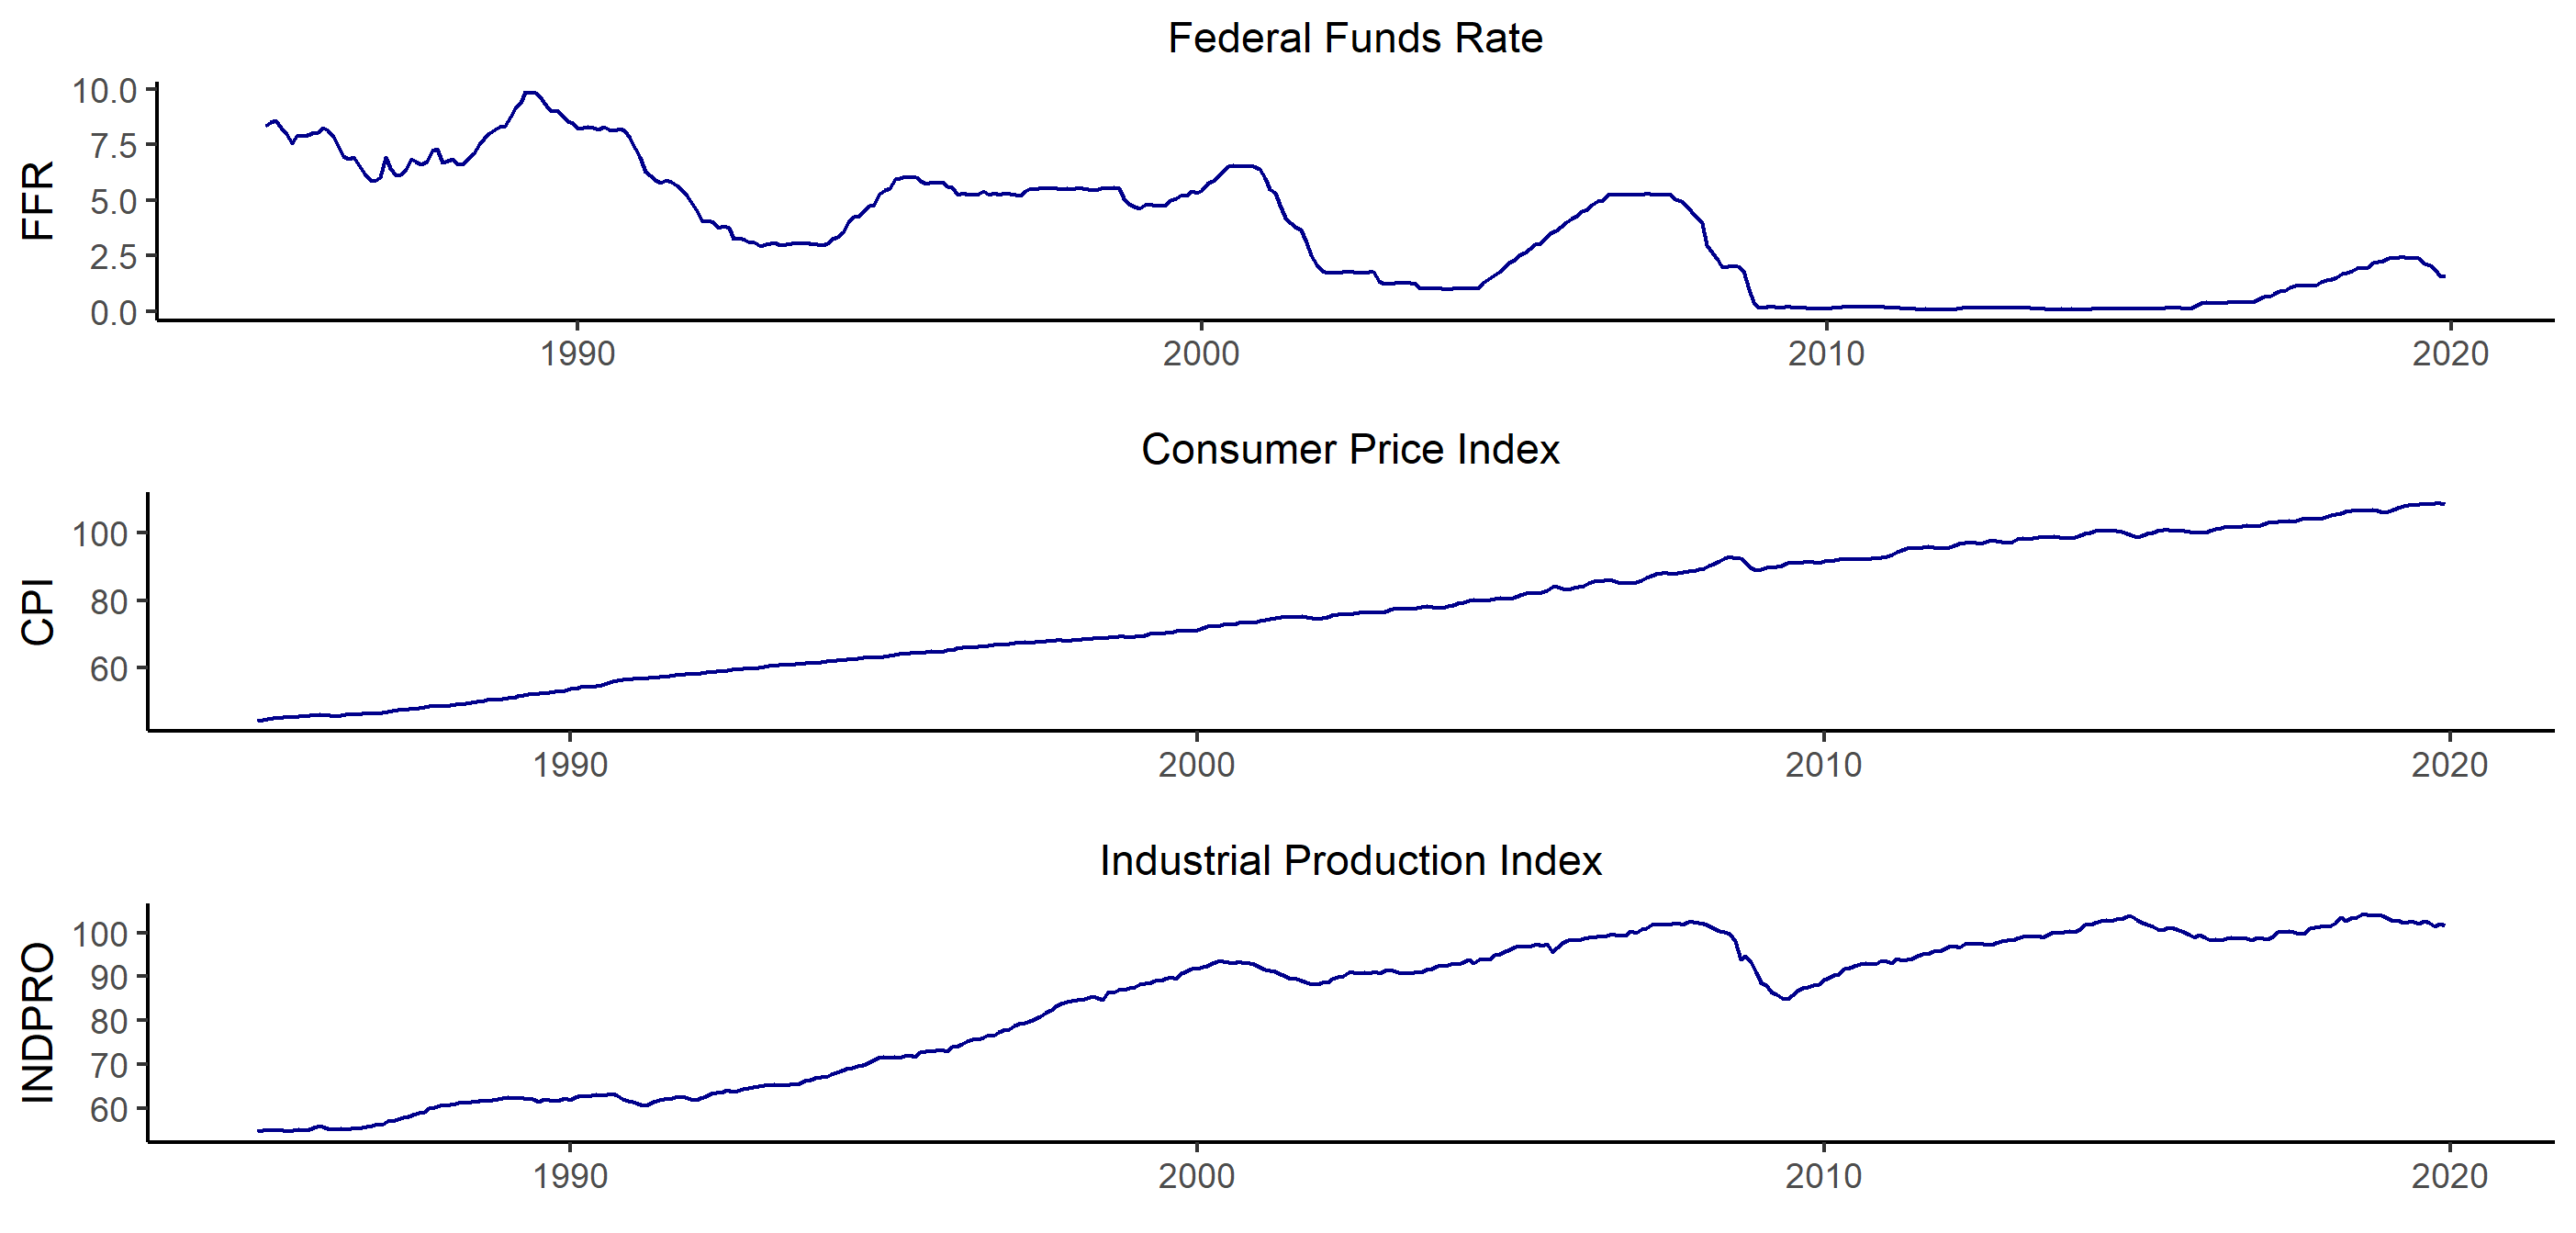
\includegraphics[width=0.9\linewidth]{plot1.png}
		\caption{Time series plots of the Federal Funds Rate, Consumer Price Index and Industrial Production Index for the USA.}
\end{figure}
\end{center}

As most macroeconomic variables, these data series are not stationary either, which is not desirable for the stability of the VAR models. For this reason I will be using the first difference of the industrial production index and the CPI. However, I will use the FFR at its level. This way I have better stability in my models and all variables have clear economic interpretation, as the two first-differenced data series can be considered as monthly growth rates of production and inflation respectively.\\

Another key variable I will be using as a "quasi transition variable" is a measure of uncertainty. This however is not a trivial metric, as several data series can be interpreted as a measurement of economic turmoil. The most commonly used are among others the VIX index and the TED spread. 
\begin{center}
	\begin{figure}[h!]
		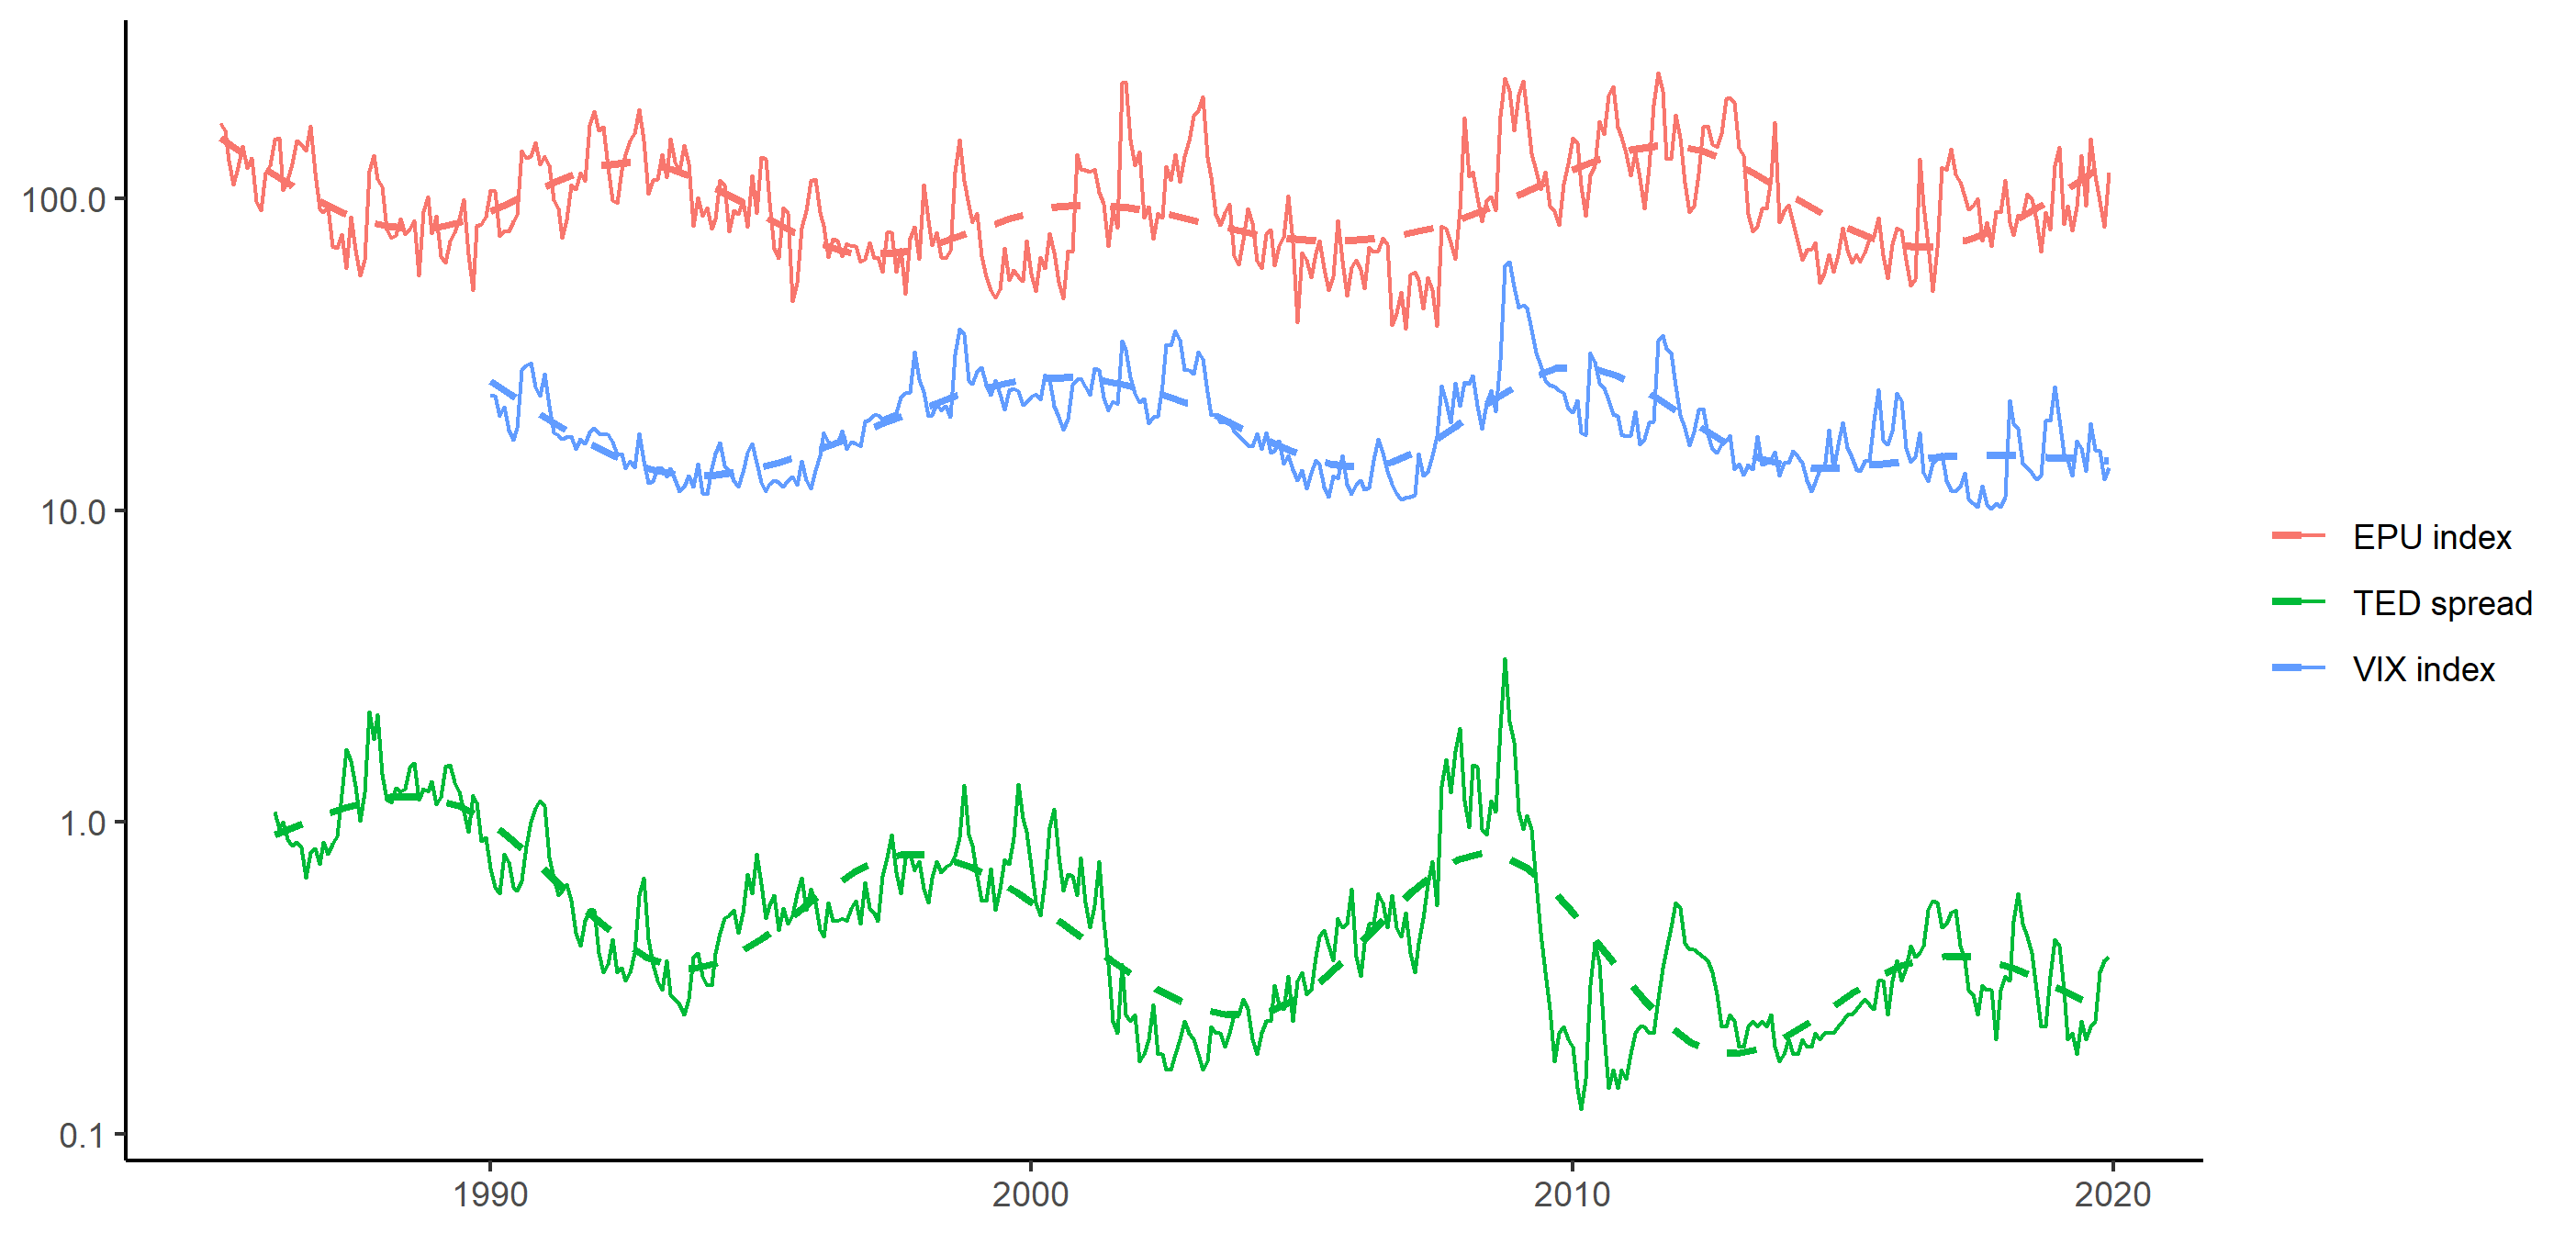
\includegraphics[width=0.9\linewidth]{plotcompare.png}
		\caption{Time series plots of the VIX index, TED spread and the Economic Policy Uncertainty index, log scales.}
	\end{figure}
\end{center}
The former derives from the market expectations on the price changes of the S\&P500 index, while the latter is the difference between the 3 month London interbank rate and the 3 month US treasury bill. Both are widely used in measuring financial stress or uncertainty, however in recent years in the literature on uncertainty, news based indices have gained a lot of traction. One such is the Economic Policy Uncertainty index created by \textcolor{blue}{\cite{baker2016measuring}}. 

\begin{center}
\begin{figure}[h!]
	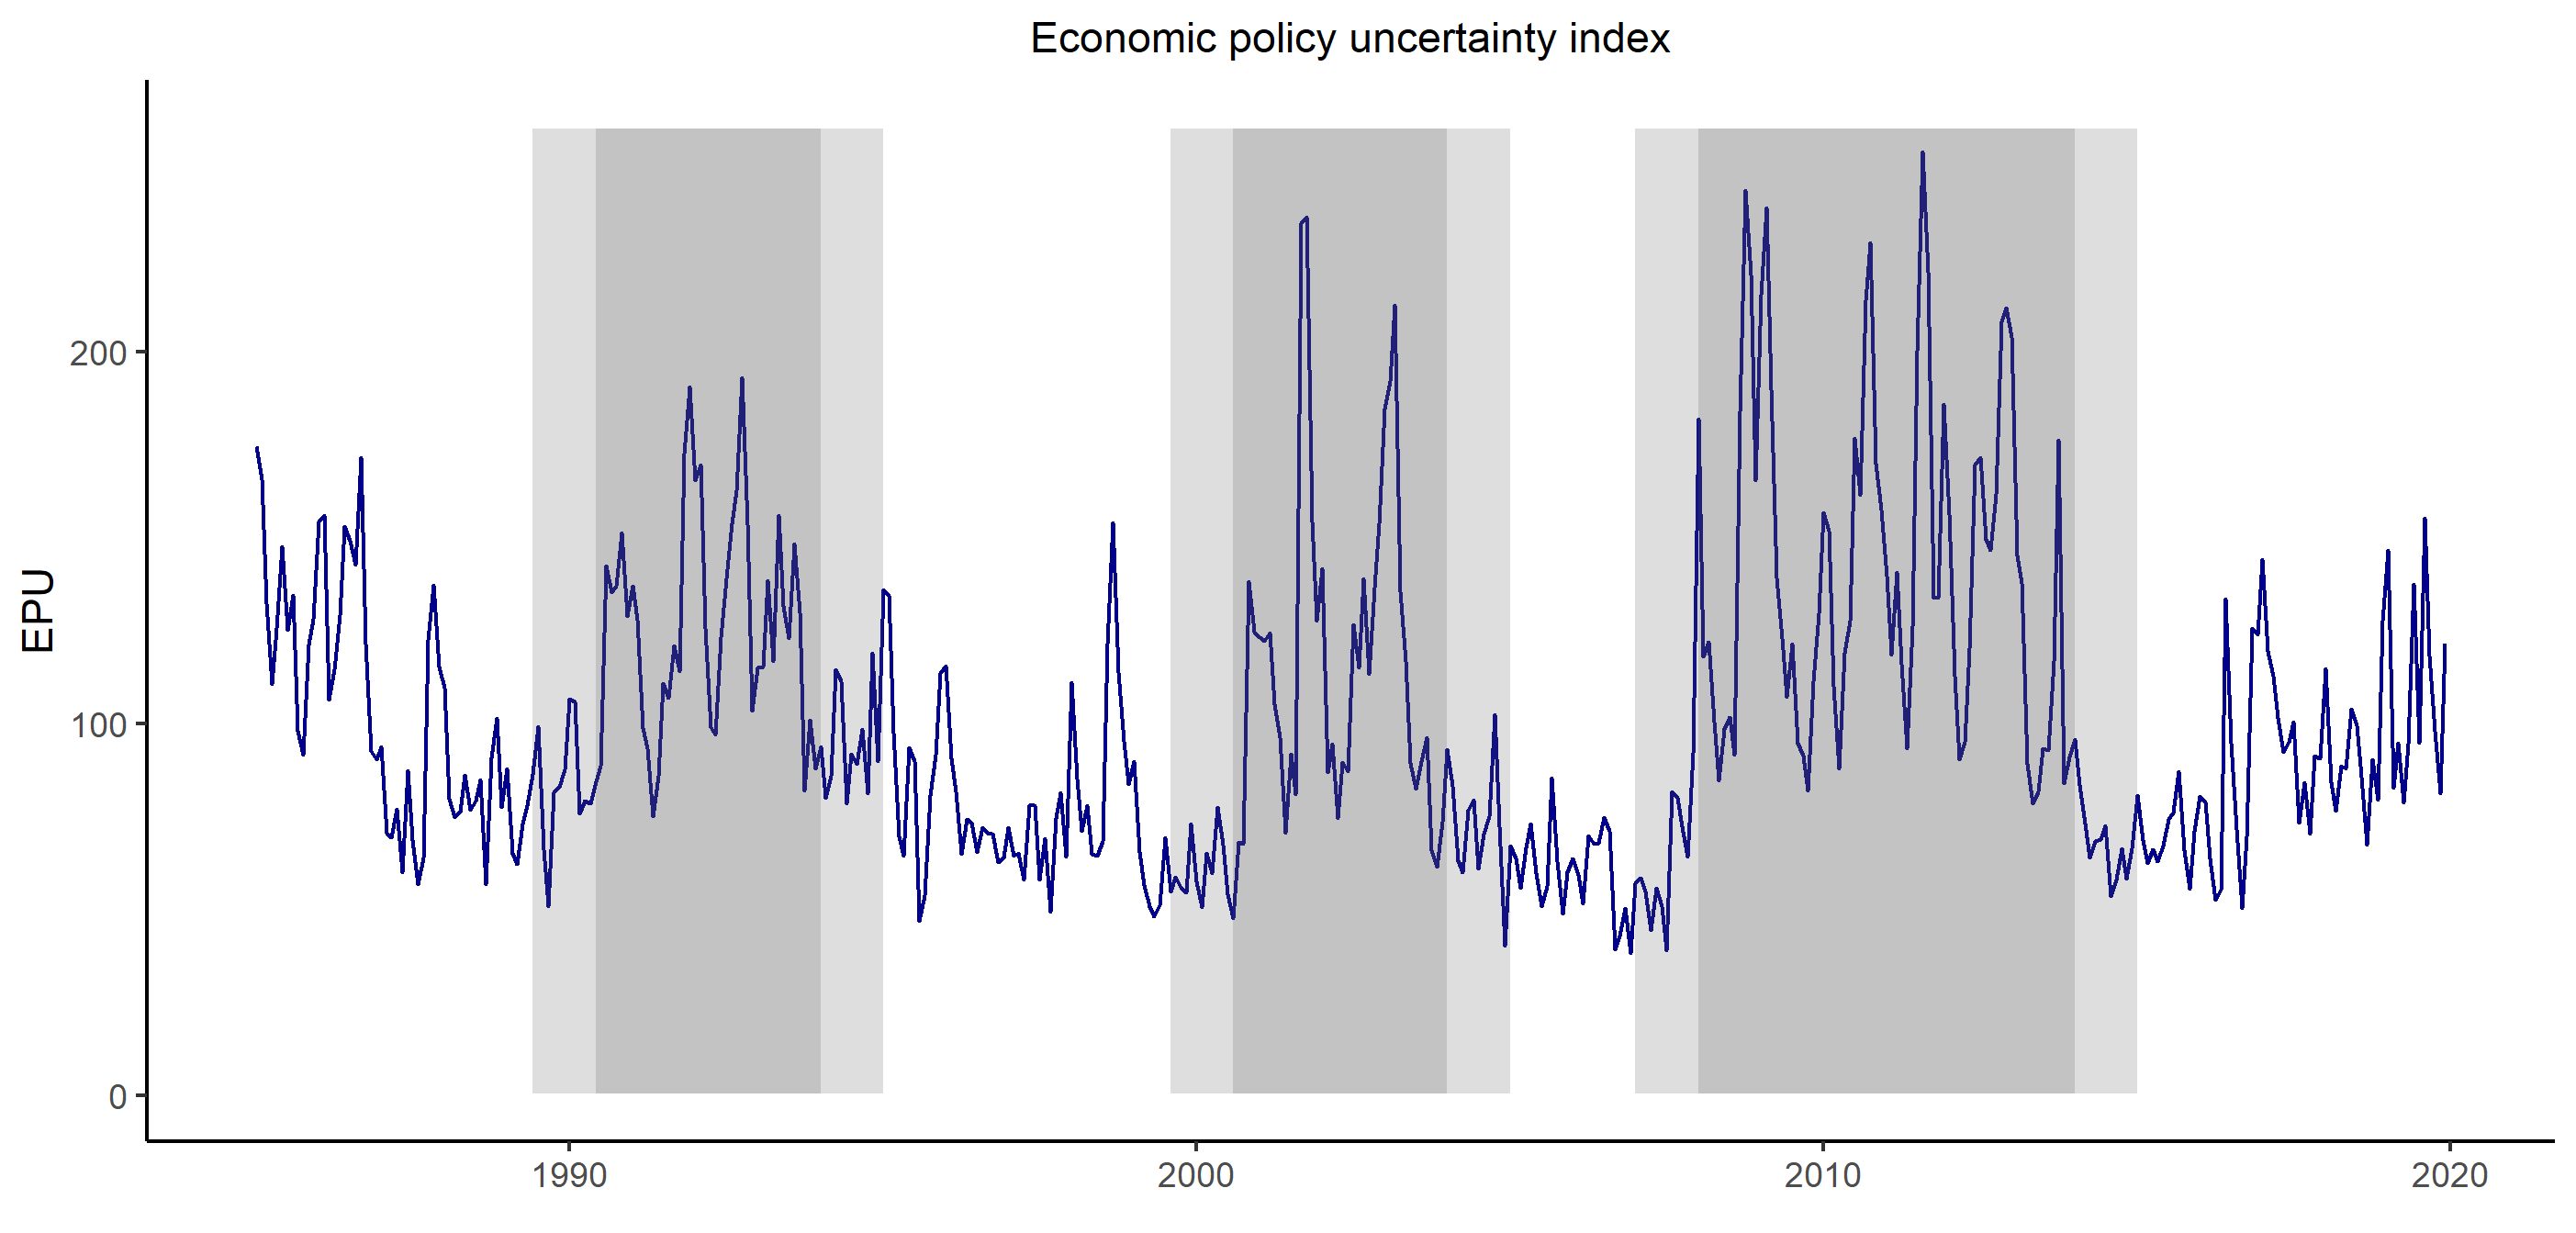
\includegraphics[width=0.9\linewidth]{epu.png}
		\caption{Time series plot of the BBD Economic Policy Uncertainty Index. The shaded areas indicate time periods with high uncertainty spikes over which the Bayesian VAR models will be estimated for the purposes of this analysis.}
\end{figure}
\end{center}
\noindent The index is primarily news based, on uncertainty related keywords in influential papers in the US. The index also takes into account temporary tax measures reported by the Congressional Budget Office and the dispersion of individual forecasts from the Federal Reserve Bank of Philadelphia's Survey of Professional Forecasters in the consumer price index and government expenditure. The index is constructed by normalizing the sub-components by their respective standard deviation and the normalized series weighted averaged (with the news based component having the highest weight of 0.5). As this index 1) covers a broader spectrum of expectations than the financial market based uncertainty counterparts, and 2) is more specific to economic policy, I believe it should serve as the most adequate measurement of uncertainty for the purposes of this study.\\

In order to estimate the asymmetric effect of uncertainty on monetary transmission, I will be estimating sign restricted VAR models over periods with high uncertainty spikes. These time periods are July 1990 - January 1994,  August 2000 - January 2004, and January 2008 - January 2014. In order to have a sufficient amount of data points, I will also include 12-12 months before and after these periods, as shown with a lighter gray highlight in the graph above.
	
\section{Empirical strategy}
An empirical challenge for this analysis was coercing the macroeconomic aggregates to behave the way it is written in all macroeconomics textbooks, i.e. to solve the price puzzle. 
There have already been numerous papers on the topic of solving the price puzzle (e.g.: \textcolor{blue}{\cite{RePEc:eee:moneco:v:51:y:2004:i:7:p:1385-1413}}, \textcolor{blue}{\cite{RePEc:hhs:hastef:0414}}, \textcolor{blue}{\cite{RePEc:spr:empeco:v:46:y:2014:i:2:p:701-731}}, \textcolor{blue}{\cite{RePEc:rba:rbardp:rdp2017-02}}, \textcolor{blue}{\cite{RePEc:aea:aejmac:v:8:y:2016:i:4:p:75-102}}, \textcolor{blue}{\cite{RePEc:aea:aecrev:v:94:y:2004:i:4:p:1055-1084}}), however with the available data series the best empirical approach would be to apply sign restrictions in the model specification. For this purpose, I will be estimating Bayesian VAR models closely following \textcolor{blue}{\cite{RePEc:eee:moneco:v:52:y:2005:i:2:p:381-419}} with a non-informative Gaussian inverted-Wirshart prior. The computation is done by implementing the R package created by \textcolor{blue}{\cite{Danne2015}}. More specifically, out of the two methods proposed, I will be using the "penalty" algorithm instead of the "rejection" algorithm. The latter one is constructed to only accept simulations that exactly satisfy the given sign restrictions, while in the former case, the goodness of fit is also taken into account. This method finds the results that are as close to satisfying the sign restrictions by minimizing a function that penalizes the impulse responses that do not meet the sign restrictions imposed.\\ 

This empirical strategy however is by no means perfect. The use of sign restricted vector autoregressive models can be criticized for artificially creating the desired model structure. For this, at the time of submitting, I have no solution, as the results would not be robust to a non-restricted model specification due to the price puzzle effect. Another disadvantage of using the sign restriction method is that the system of shocks is not completely identified. This however, is not a major issue in this paper, as only the identification of a shock to the Federal Funds Rate is necessary.\\

In order to be able to find asymmetries in monetary transmission, I will first need a basis for comparison. For this purpose, I will first estimate a baseline model over the whole available time period. Next, I will estimate a number of models in a 5 year (12 month) rolling window over time periods highly affected by uncertainty spikes. All models will be of lag order 1, and the reduced form VAR model can be written as:
\begin{equation}
	B(L)Y_{t} = \alpha_{0} + \epsilon_{t},
\end{equation}
where  $B(L)$ is the matrix of coefficients for at lag L, $Y_{t}$ is the vector of endogenous variables, $\alpha_{0}$ is the vector of constants and $\epsilon_{t}$ is the error term. The ordering of the variables will be
\begin{equation}
	Y_{t} = 
	\begin{Bmatrix}
		FFR_{t} \\
		CPI_{t} \\
		INDPRO_{t}
	\end{Bmatrix}
\end{equation}
\noindent which if important for decomposition, as in the algorithm used, the first variable is considered the shock variable (this is given a positive sign restriction) and the sign restriction of the following variables is set accordingly (negative in both cases).\\

In order to compare and analyze results, I find the use of impulse responses to be the best tool. For the baseline model, this is a quite straightforward process, but for the rolling window estimates, some aggregation will be required. For this purpose, I will be taking point-by-point medians from impulse responses of each estimated model.

\section{Results}
To be able to compare results, first we must define the effectiveness of the monetary transmission mechanism. For our purposes, I will consider the mechanism more effective the better it is at anchoring inflation at a smaller trade-off in economic activity. In other words, the higher impact on the CPI inflation and a lower impact on the industrial growth index.\\

Figure 3 below shows the impulse responses from the benchmark model (first row) and from the rolling window estimation (second row). From the graphs we can see that the impact of the interest rate shock to inflation is quite similar in both cases, with the response in the benchmark model being slightly more persistent. Looking at the FFR shock's response to a shock to itself might give an explanation. We can see that the estimated shock in the baseline model is much larger in volume and much more persistent compared to the results from the rolling window estimation. This by itself is an interesting outcome (which I will get to later), however this seems to partially contradict my prior beliefs, as the relative impact of the shock to inflation would be larger in uncertain times. Looking at the impulse responses of the industrial growth index, we can see a more minor but somewhat more persistent response in the baseline model comparing to the rolling window median response. As to the persistence, a similar explanation can be given, however the drop in output is much sharper in the latter case, which confirms my prior assumption that an interest rate shock during higher uncertainty would slow down the economy much more, thus being less effective. As mentioned before, an interesting result is the path of the FFR shock. In the baseline estimate, the shock seems to be rather persistent, 

\begin{center}
\begin{figure}[h!]
	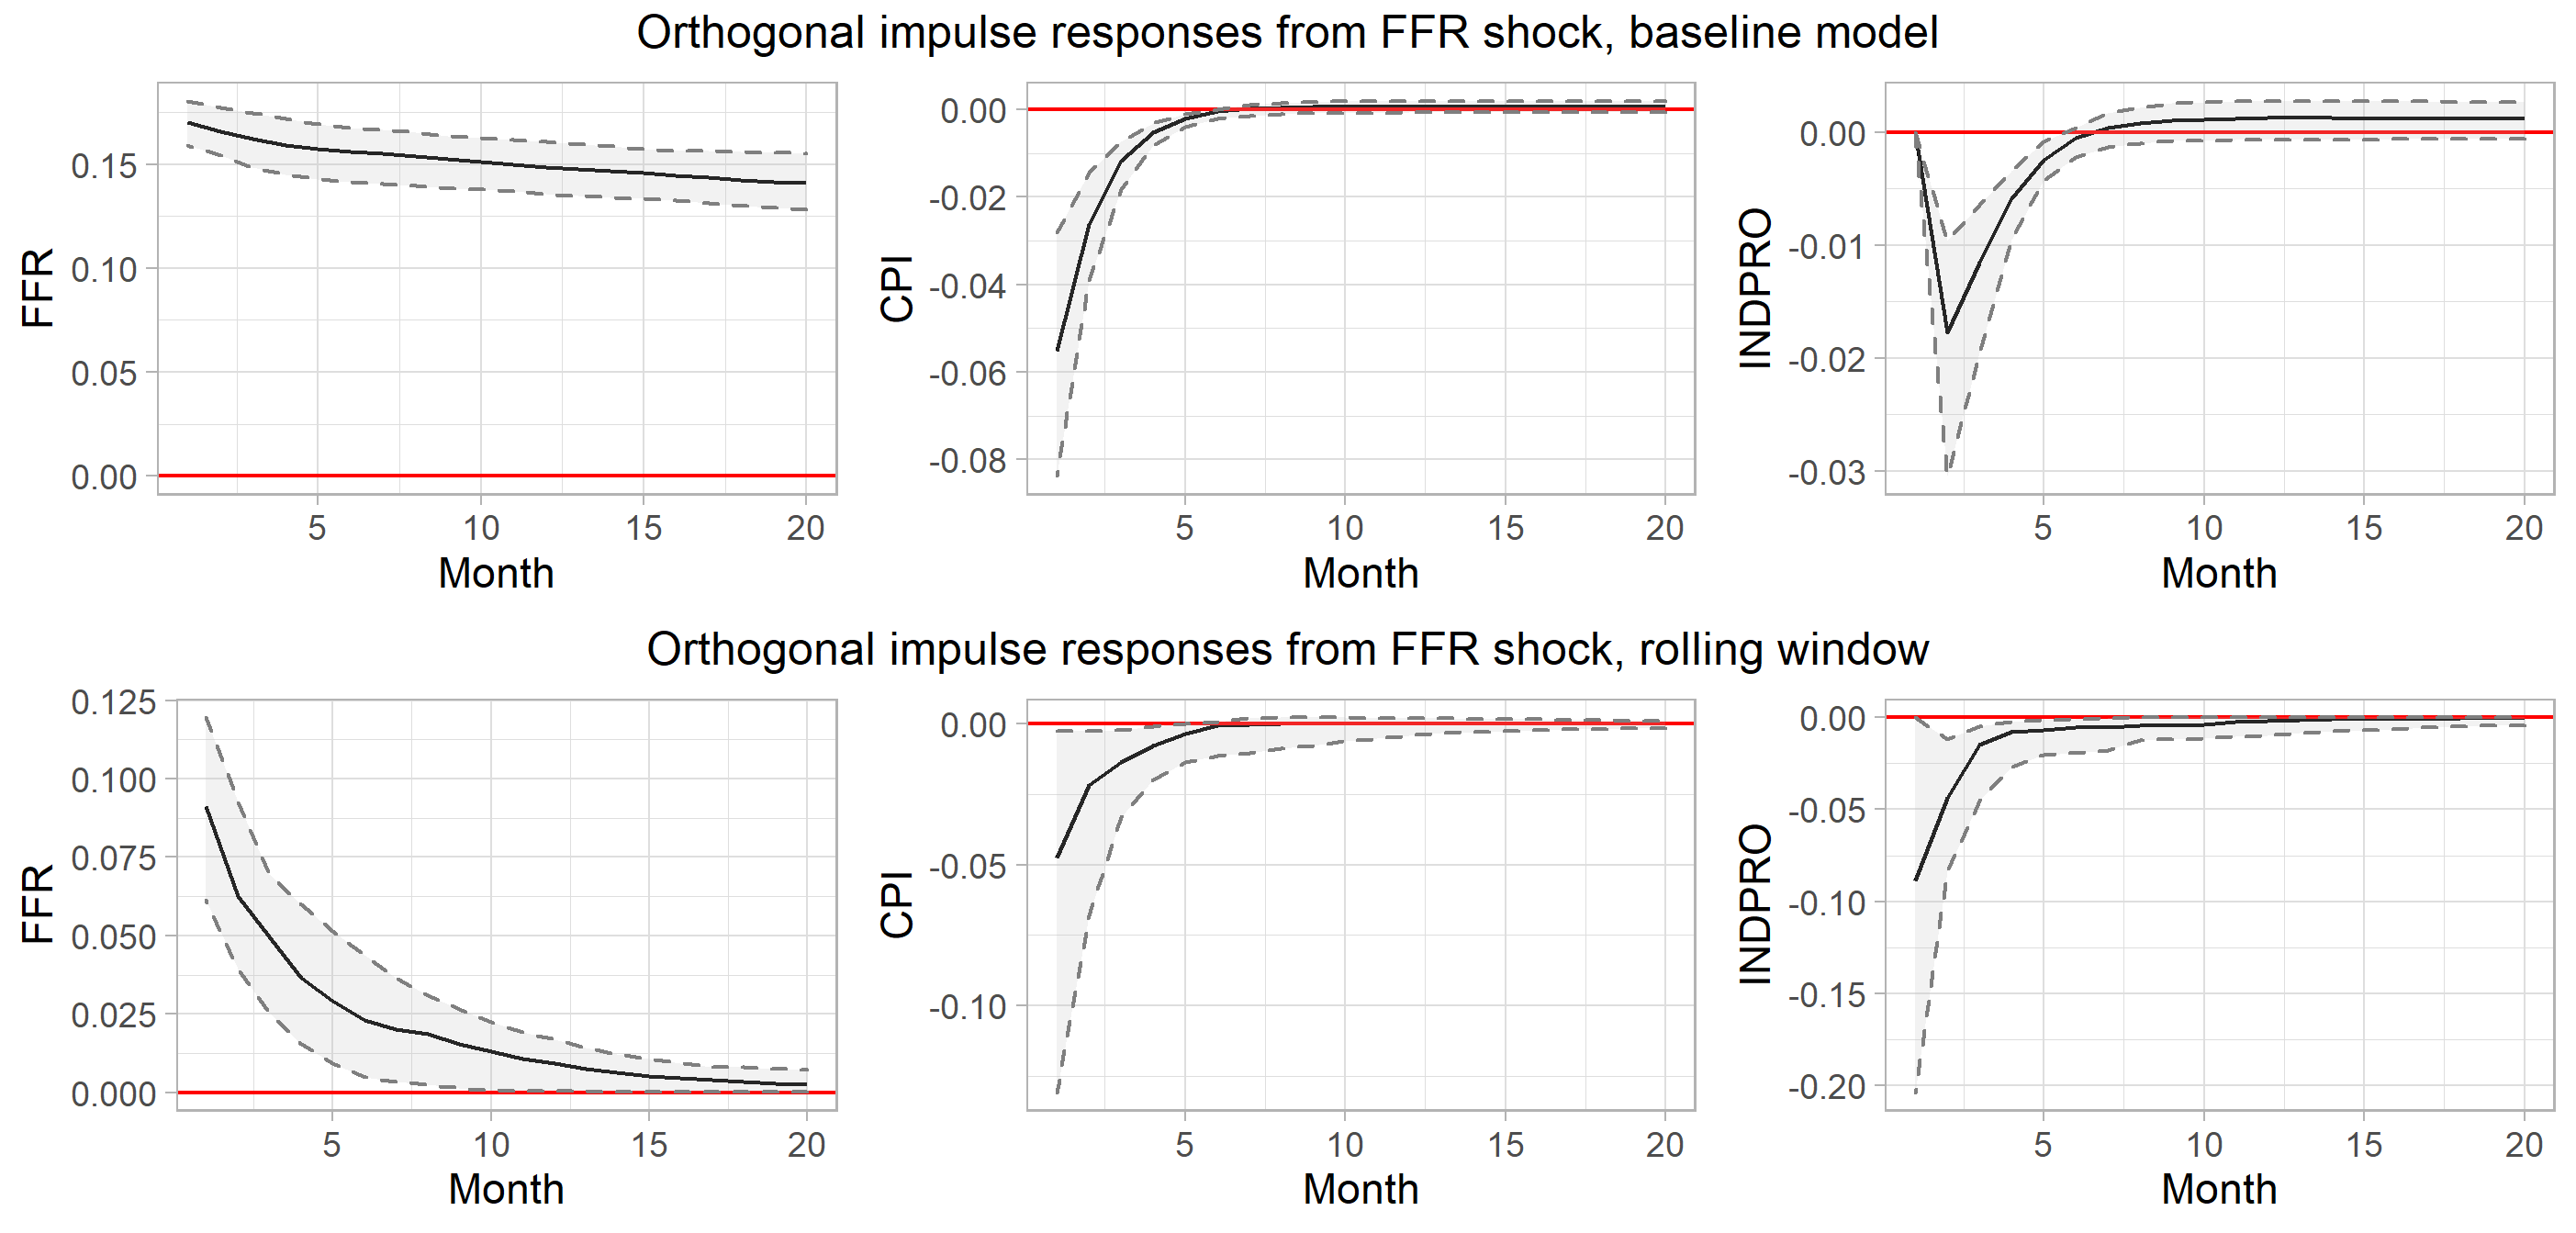
\includegraphics[width=0.9\linewidth]{irfplot1.png}
			\caption{Impulse responses from the benchmark model (first row) and median impulse responses from the rolling window estimation (second row).}
\end{figure}
\end{center}
\noindent indicating a near extreme interest rate smoothing by the Federal Reserve in a general setting, however, in the second case the shock decays much faster, which could indicate - similarly to recession periods - a more active policy style with less focus on smoothing interest rates. This could mean that not only could there be asymmetric effects of monetary policy during periods of high uncertainty, but policy making could also be asymmetrical, similarly to the propositions of \textcolor{blue}{\cite{doi:10.1080/1331677X.2018.1481445}}.\\



To further investigate, I will also be taking a look at the decomposition of the median impulse responses of the rolling window, by taking separate median impulse responses for each of the three highlighted time periods. This can be seen in Figure 4 below.   
\begin{center}
\begin{figure}[h!]
	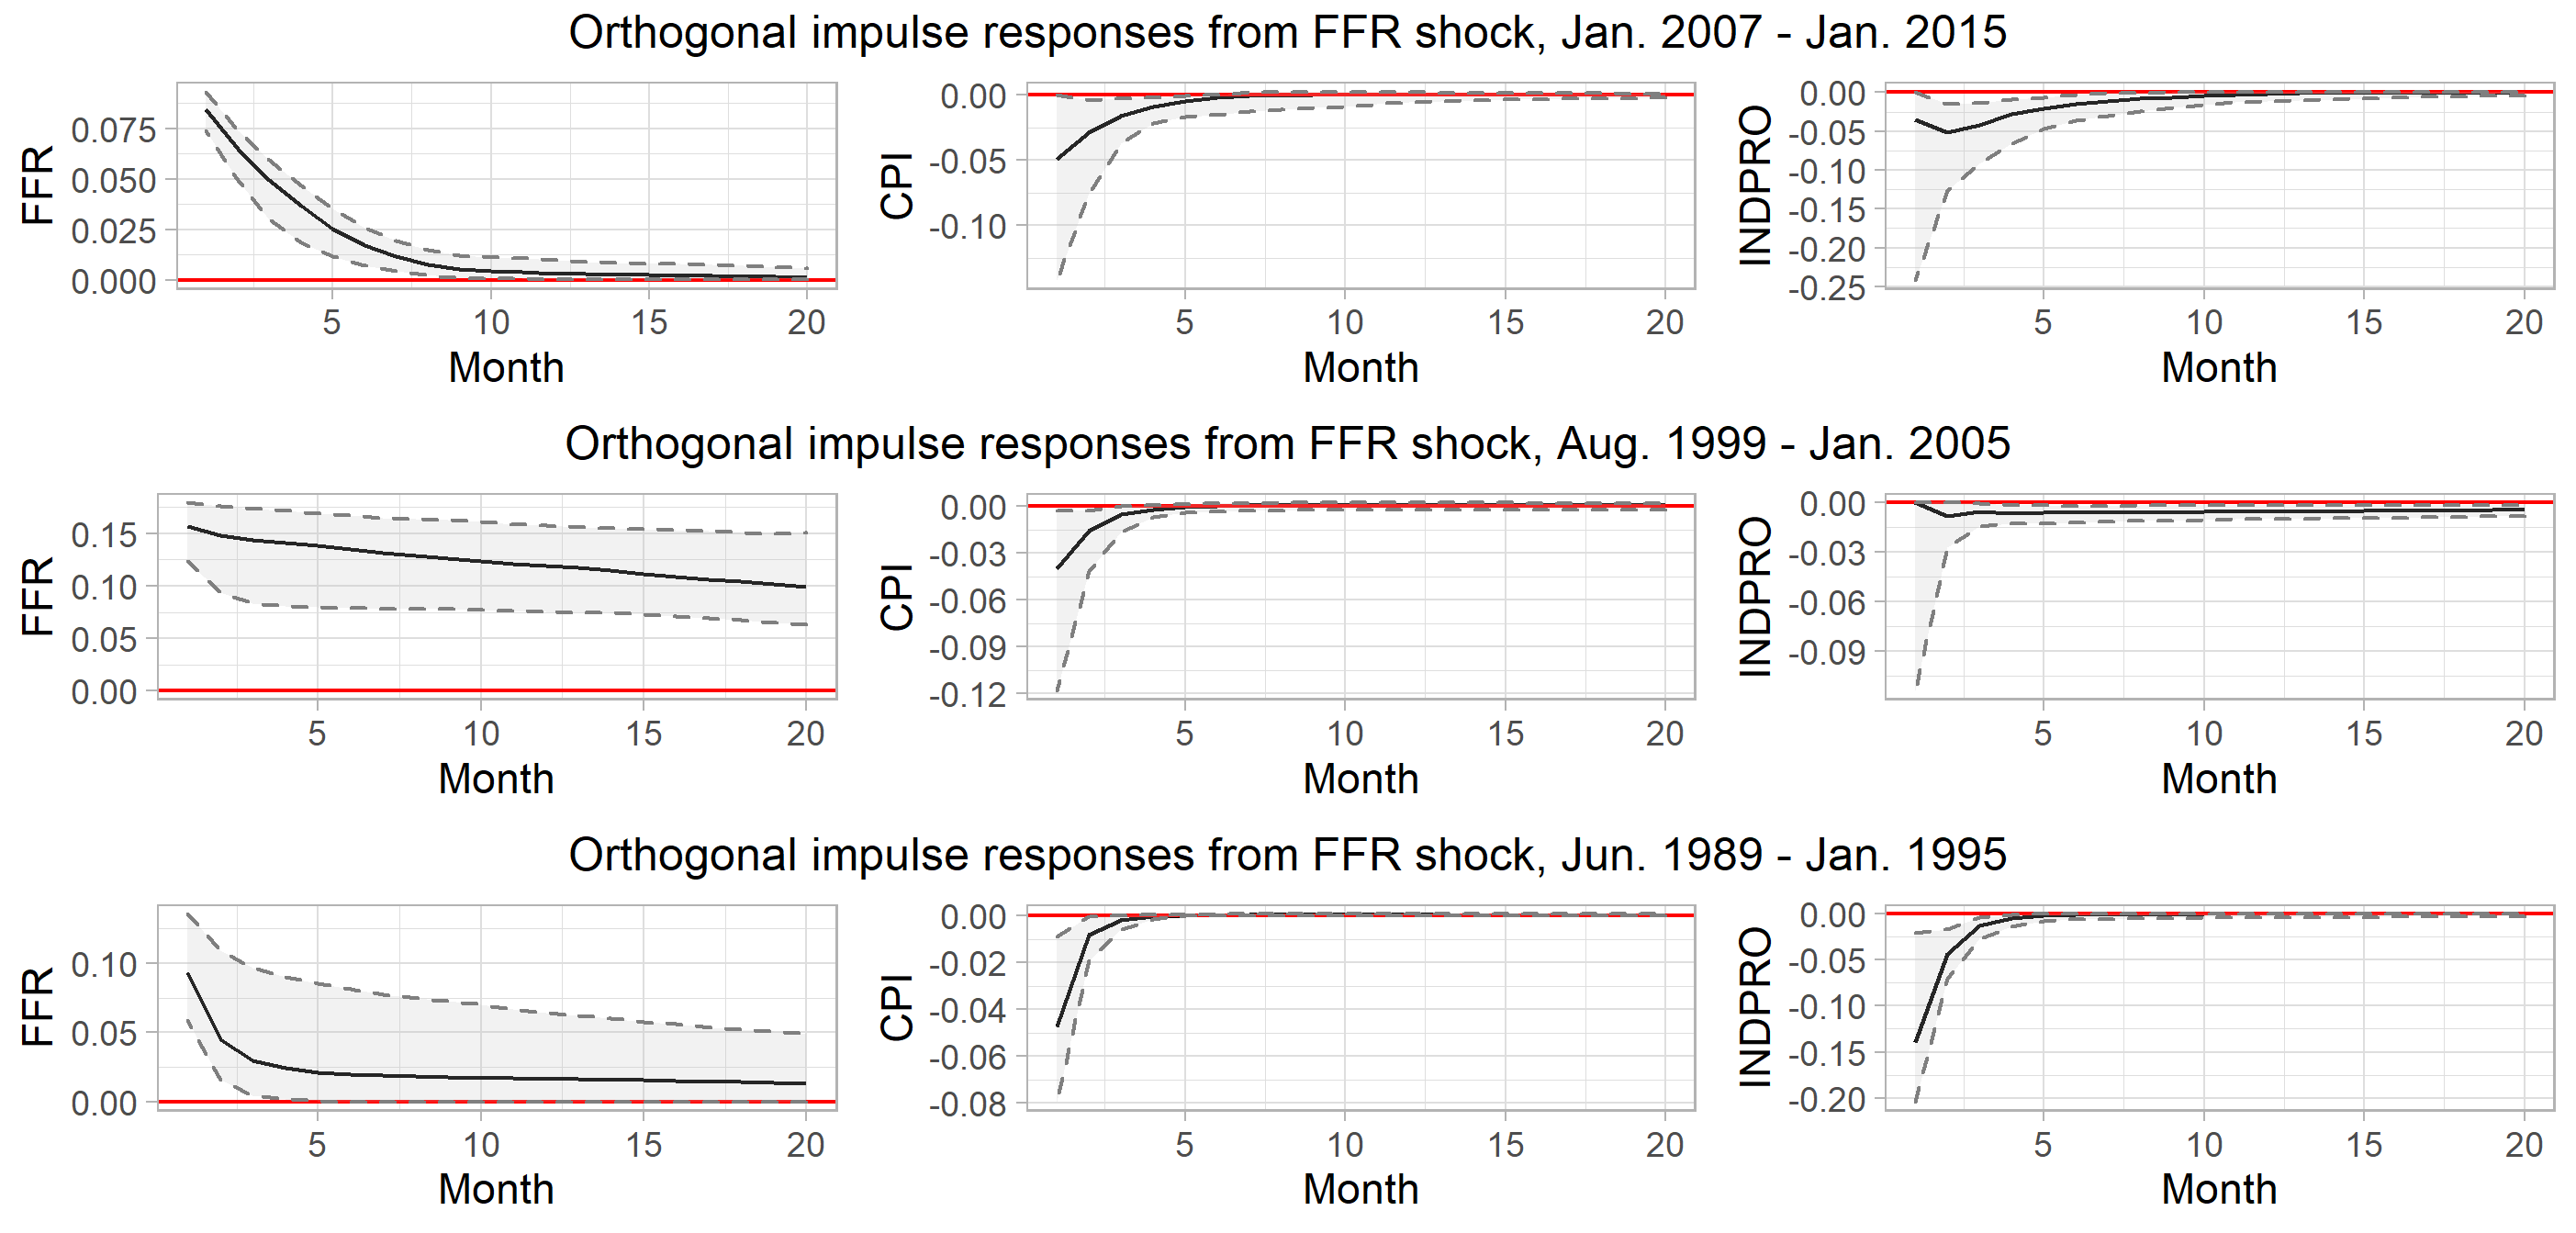
\includegraphics[width=0.9\linewidth]{irfplot2.png}
			\caption{Separate median impulse responses from rolling widow estimation over the three high-uncertainty periods.}
\end{figure}
\end{center}
By taking a look at the separate IRF-s, we get mixed results. While the uncertainty spikes in each period are similar in volume and pattern, the impulse responses can differ substantially.\\ 
\noindent During the period January 2007 - January 2015, the reasons for uncertainty are pretty self explanatory, as most of this time period is characterized by the devastating economic impact and aftermath of the Great Recession. An explanation as to why the uncertainty index was volatile for such a great length could be the Euro Area crisis which followed shortly after the Great Recession. As Europe is one of the most important trading partners of the US, the overseas crisis must have gained substantial news coverage in the US as well, which would by design cause the index to rise considerably. In the impulse response graphs, we see a fast decaying shock and responses similar to the baseline case in inflation and industrial growth. The path of the FFR response could be explained by the active policy making at the beginning of the period - as it was necessary during the Great Recession. \\
\noindent In the case of time period August 1999 - January 2005, an explanation of higher uncertainty could be the fact that the industrial growth peaked in the early 2000s, after which we see a brief decline. The peak in output is usually considered the end of a boom cycle, and a start of a recession, which could cause a surge in uncertainty. During this period we see a relatively steady growth in CPI, however there were major interest rate cuts in the beginning of the century as a reaction to the signs of economic decline - another reason for the uncertainty index to spike. Following these first few years, the FFR was kept steadily at a rate of about 2.5\%. The estimated responses of inflation and industrial growth in this period are nearly negligible, which could possibly indicate the lack of effect of monetary policy during non/mild-recession times. 
\noindent The explanation for high uncertainty in the period June 1989 – January 1995 is similar to the previous case, as we can see the industrial growth reaching a local maximum in the early 90s. The economic contraction was primarily caused by tightening monetary policy, as we can also see rates hike in Figure 1. Another cause for the contraction was the Tax Reform Act of 1986, leading to a bust in growing real estate prices, thus also disincentivizing investments. The economy coming to a downward shift, the monetary policy tightenings and the tax reform bill altogether would cause much news coverage as well, which by construction causes the EPU index to soar. An interesting observation of this period is that the sharpest drop in inflation and industrial growth can be observed in the impulse responses, as inflation drops by close to 5 percentage points and the industrial growth index drops by an outstanding amount of close to 12 percentage points. The reason why the economic impact of an interest rate shock is much more severe compared to other time periods could be by the underlying economic theory “losing its explanatory potential”, as in later times the key drivers behind the business cycle could be shifting to factors not included in economic models. All in all, we can see close to no asymmetry in the effect of monetary transmission on the inflation rate, and a minor asymmetric effect on output.

\section{Conclusion}
In this paper, I aimed to find asymmetries in the monetary transmission mechanism in high-uncertainty times. For this purpose, I estimated several sign restricted VAR models in five-year rolling windows, and a sign restricted model as baseline. In the results of the estimation, I found close to no asymmetry in the effects of an interest rate shock to inflation, however there is a minor difference in how it impacts output, as the drop in industrial growth in noticeably sharper during periods of high uncertainty. While the results are minor, they have a somewhat important policy making aspect. More specifically, it highlights the importance of forward guidance measures alongside interest rate decisions as a counter-measure to higher economic uncertainty in order to mitigate its effect on the contraction of economic growth. 

\printbibliography[title = References]
	
	
\end{document}